\documentclass[headings=standardclasses,headings=big,oneside,a4paper,openany,12pt]{scrbook}

\newcommand {\e}[1]{\mathrm{~#1}}
\newcommand {\E}[1]{\times 10^{#1}}
\newcommand {\vars}{$\Delta E$ and $M_{BC}$}
\newcommand {\btbii}{\texttt{B2BII}}
\newcommand {\decaya}{$B \to K K \ell \nu$}
\newcommand {\decayb}{$B^+ \to K^+ K^- \ell^+ \nu$}

%\usepackage{biblatex}
%\bibliography{mybib.bib} 
\usepackage[slovene,english]{babel}% Recommended
\usepackage{csquotes}% Recommended
\usepackage[sorting=none,firstinits=true,backend=bibtex]{biblatex}
\addbibresource{mybib.bib}% Syntax for version >= 1.2

\usepackage{paralist}
\usepackage{caption}
\usepackage{cancel}

\usepackage{longtable}

\setlength{\parskip}{1em}%
\setlength{\parindent}{0cm}

\usepackage{titling}
\usepackage{amsmath,amssymb,amsfonts,nicefrac}
\usepackage{graphicx}
\usepackage{color}
\usepackage{float}
\usepackage{mathtools}
\allowdisplaybreaks
\usepackage[pdftex,colorlinks=true,citecolor=blue,linkcolor=black,urlcolor=blue,bookmarks=true]{hyperref}
\usepackage{dictsym}
\usepackage{braket}
\usepackage{slashed}
\DeclareMathOperator{\arcsinh}{arcsinh}
\usepackage{enumerate}
\usepackage{array}
\setlength{\extrarowheight}{.5ex}

\usepackage{lineno}
\linenumbers

\usepackage{subfigure}


\begin{document}
\begin{otherlanguage}{slovene}
\chapter{Povzetek doktorskega dela}

\section{Uvod}
Fizika delcev je eden od stebrov fizike, z mo"cnimi koreninami, ki segajo vse do začetka 20. stoletja. Natan"cni eksperimenti in preverljiva teorija so pokazali, da vesolje sestoji iz osnovnih delcev in nosilcev interakcij. Osnovne delce delimo na kvarke ($u$, $d$, $s$, $c$, $b$, $t$) in leptone, ki so nadaljnje razdeljeni na nabite leptone ($e$, $\mu$, $\tau$) in pa nevtrine ($\nu_e$, $\nu_\mu$, $\nu_\tau$). Nosilci štirih osnovnih interakcij so fotoni ($\gamma$) za elektromagnetno, gluoni ($g$) za močno in nabiti- ($W^\pm$) ter nevtralni ($Z^0$) bozoni za šibko interakcijo. Vse delci imajo maso, ki jim jo določa Higgsov bozon ($H$). Vse delce ter interakcije med njimi opisuje Standardni model, ki je osrednja teorije fizike visokih energij. Kvarke lahko združujemo v kombinacije oblike $q_1 q_2 q_3$ (hadroni) ali pa $q_1 \bar{q}_2$ (mezoni), med katere sodijo tudi protoni in nevtroni, ki jih opazimo v naravi. Poleg omenjenih dolgo-živečih delcev pa obstajajo tudi težji, bolj nestabilni delci, ki preko zgoraj naštetih interakcij razpadejo v lažje, stabilnejše. Raziskovanje takšnih procesov s pomočjo pospeševalnikov in trkalnikov nam omogoča spoznati zakone vesolja vse od danes pa do njegovega začetka.

Osrednji del doktorske disertacije predstavljajo mezoni $B$, delci, ki so sestavljeni iz težkega kvarka $b$ in enega od lahkih kvarkov $u$ ali $d$. Ena od bolj presenetljivih lastnosti vesolja je kršitev simetrije $CP$, t.j. kombinacije simetrij konjugacije naboje ($C$) in prostorske inverzije ($P$). Simetrija $CP$ nakazuje, da so fizikalni procesi delcev in zrcalni procesi antidelcev enaki, kar pa danes vemo, da ne drži v celoti in poznamo procese, ki to simetrijo kršijo. Kršitev simetrije $CP$ je tesno povezana s šibko interakcijo, to pa predstavlja našo motivacijo za študijo mezonov $B$, saj šibki razpadi predstavljajo večji del razpadov mezonov $B$.

Edinstvena lastnost šibke interakcije je, da lahko spreminja tip oziroma t.i. okus kvarkov, medtem ko ga ostale interakcije ohranjajo. Takšni procesi so opisani s prehodno matriko CKM (Cabibbo-Kobayashi-Maskawa) \cite{cabibbo1963unitary,kobayashi1973cp}
\begin{equation}
V_{CKM} = \begin{bmatrix}
    V_{ud} & V_{us} & V_{ub}\\
	V_{cd} & V_{cs} & V_{cb}\\
	V_{td} & V_{ts} & V_{tb}
\end{bmatrix}.
\end{equation}
Unitarnost matrike CKM nam omogoča, da iz nje izluščimo matematične identitete, od katerih je ena od pomembnejših
\begin{equation}
V_{ud}V_{ub}^* + V_{cd}V_{cb}^* + V_{td}V_{tb}^* = 0,
\end{equation}
ki je poznana pod imenom unitarni trikotnik, saj predstavlja zaključen vektor treh točk v kompleksni ravnini, ki ga prikazuje Slika \ref{fig:ut_si}. Parametri matrike CKM niso določljivi s strani teorije, temveč jih moramo določiti z eksperimentalnimi meritvami tako, da najdemo procese, ki so tesno povezani s stranicami in kotni unitarnega trikotnika. Na tak način lahko preverimo, če je oblika trikotnika konsistentna, kar predstavlja dober test Standardnega modela, oziroma če so potencialno prisotni kakšni novi procesi, ki jih še ne poznamo, in jih kolektivno imenujemo "nova fizika". Dodatna motivacija za študijo mezonov $B$ je ta, da velik delež njihovih razpadov predstavlja koristne procese za meritev unitarnega trikotnika.
\begin{figure}[H]
\centering
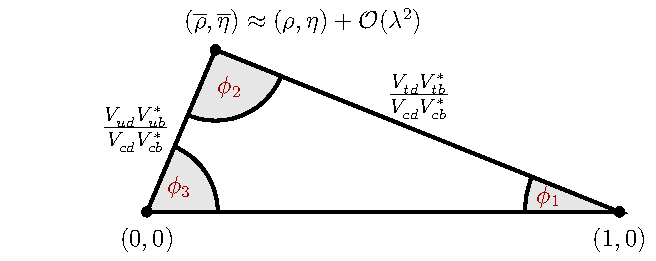
\includegraphics[scale=1]{texfig/UT_Triangle}
\caption{Unitarni trikotnik s parametri $\lambda,~\eta,~\rho$ and $A$ (slednji ni prikazan), ki predstavljajo proste parametre matrike CKM.} %TODO: Wolf. param. 
\label{fig:ut_si}
\end{figure}

Procesi, ki jih študiramo v tej analizi, so tesno povezani z elementom $V_{ub}$ matrike CKM, saj le-ta opisuje prehode kvarkov $b \to c$. Od vseh elementov, je absolutna vrednost tega elementa najmanjša, relativna napaka pa največja, zato meritve iz tega področja potencialno omogočajo največ izboljšave. Such quark transitions are present in charmless semi-leptonic $B$ meson decays of the form
\begin{equation}
B^+ \to X_u^0 \ell^+ \nu_\ell,
\end{equation}

where $X_u^0$ represents a charmless hadron with a $u$ quark and $\ell$ is one of the charged leptons $e,~\mu$ or $\tau$. Measuring the decay rate of the $B$ meson in such decays paves the way for the CKM matrix element determination. Decay rates are directly connected to the $V_{ub}$ element as
\begin{equation}
\mathrm{d} \Gamma \propto G_F^2 \vert V_{ub} \vert ^2 \vert L^\mu \langle X_u \vert \bar u \gamma_u \frac{1}{2} (1-\gamma_5) b \vert B \rangle \vert ^2,
\end{equation}

where $\Gamma$ is the decay width, $G_F$ is the Fermi coupling constant, $L^\mu$ is the leptonic current and the expression in the Dirac brackets is the hadronic current. The factor $\vert V_{ub} \vert ^2$ represents the probability for the $b \to u$ quark transition. Measurement of the $V_{ub}$ CKM matrix element can be performed in two possible ways. With the exclusive or the inclusive method, which are described below. Both methods require different experimental and theoretical techniques, so they provide largely independent determinations of $\vert V_{ub} \vert$. Currently both methods also have comparable accuracies. 

In the exclusive method one studies the decays of $B$ mesons to a specific charmless hadronic final state, such as $B \to \pi \ell \nu$. Clean determination of the $V_{ub}$ is possible due to precise experimental measurement along with reliable theoretical calculations. However, theoretical calculations are more challenging for decays to a specific final state, since hadronization of quarks has to be taken into account. There are also two main experimental challenges in this method. One has to reduce the abundant background from $B \to X_c \ell \nu$ processes, since the $b \to c$ quark transition is much more common. The second experimental challenge is to separate the $B$ meson decay with the specific charmless hadronic final state from other $B \to X_u \ell \nu$ decays, since it roughly populates the same regions of the phase-space as the signal decay.

In the inclusive method one studies the decays of $B$ mesons to any charmless hadronic final state $B \to X_u \ell \nu$. In this case, the total decay rate for $b \to u \ell \nu$ can be calculated accurately, since hadronization does not have to be taken into account. The greater challenge with this method is again the experimental measurement of the total decay rate due to the $B \to X_c \ell \nu$ background. Experimental sensitivity to $V_{ub}$ is highest where $B \to X_c \ell \nu$ decays are less dominant. Theory and experiment have to compromise and limit the $V_{ub}$ determination to a region where the signal-to-background ratio is good. Theory takes this into account by reliably calculating the partial decay rate $\Delta \Gamma$, which is more challenging than the total decay rate. One possible and often used approach to reduce $b \to c$ background is to reject all events with $K$ particles, or kaons, present in the final particle selection. The procedure is called a $K$-veto. Kaons consist of an $s$ quark, which is mainly produced in $c \to s$ transitions. This means that if a kaon is found in the event, it is very likely that it originates from a particle with a $c$ quark, indicating the $b \to c$ process. 

If $V_{ub}$ is determined with both these methods, the values can be compared. It turns out that consistency between these two results is only marginal, where the difference is at a level of $3\sigma$. The current world averages \cite{Amhis:2016xyh} of the exclusive (from $B^0 \to \pi^- \ell^+ \nu$) and inclusive (GGOU collab. \cite{Gambino:2007rp}) are
\begin{align}
&\vert V_{ub} \vert_{\mathrm{excl.}} = \left(3.65 \pm 0.09 \pm 0.11\right)\E{-3},\\
&\vert V_{ub} \vert_{\mathrm{incl.}}^{\mathrm{GGOU}} = \left(4.52 \pm 0.15~{}^{+0.11}_{-0.14}\right)\E{-3},
\end{align}
where the first and the second errors are the experimental and the theoretical error, respectively. We see that inclusive measurements prefer higher values than exclusive ones. This is known as the $V_{ub}$ puzzle. It is necessary to make further research as to why this difference occurs. The reason could be an unknown experimental or theoretical error, or it is even possible that some NP contributions occur. This analysis will focus on a possible reason that could be hidden in the selection mentioned before. By performing a $K$-veto, one discards all events with kaons in the final state in order to suppress $b \to c$ contributions. In this analysis we focus on the charged \decaya~decay, which is very similar to the $B \to \pi \ell \nu$, except for a production of an $s \bar s$ quark pair, which then combines with final state quarks to form kaons, as shown in Figure~\ref{feynman}. In this case, we have kaons in the final state where the $B$ meson decayed via a $b \to u$ process. Such decays were discarded in previous $V_{ub}$ determinations with the inclusive method, but in principle they contribute to the result and should be taken into account. The results of this analysis should help us make a step closer to solving the $V_{ub}$ puzzle. 

\begin{figure}[H]
\centering
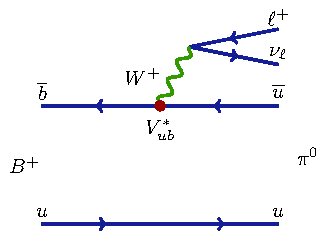
\includegraphics{texfig/B2pilnu}
\hspace{1cm}
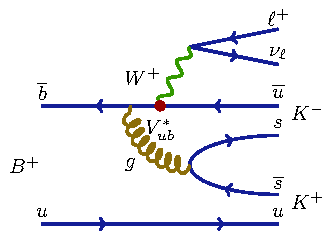
\includegraphics{texfig/B2KKlnu}
\caption{Feynman diagrams for the $B^+ \to \pi^0 \ell^+ \nu_\ell$ decay (left) and the $B^+ \to K^- K^+ \ell^+ \nu_\ell$ decay (right).}
\label{feynman}
\end{figure}

Specifically, we will be focusing on decays of the charged $B$ mesons of the form \decayb, since it includes two charged kaons, as opposed to the case of the neutral $B$ meson decay. The reason for this is a simpler decay chain and a higher reconstruction efficiency. All further occurrences of \decaya~automatically imply decays of the form \decayb~and its charge conjugated counterpart.

\section{Experimentalna postavitev}
\subsection{Trkalnik KEKB}
\subsection{Detektor Belle}
\section{Postopek analize}
\section{Sistematske negotovosti}
\section{Kon\v cni rezultat}
\end{otherlanguage}
\end{document}


